\documentclass[11pt]{article}

\usepackage[pdftex]{graphicx}
\usepackage{rotating}
\usepackage{adjustbox}
\usepackage{float}

% Use wide margins, but not quite so wide as fullpage.sty
\marginparwidth 0.5in 
\oddsidemargin 0.25in 
\evensidemargin 0.25in 
\marginparsep 0.25in
\topmargin 0.25in 
\textwidth 6in \textheight 8 in
% That's about enough definitions

% multirow allows you to combine rows in columns
\usepackage{multirow}
% tabularx allows manual tweaking of column width
\usepackage{tabularx}
% longtable does better format for tables that span pages
\usepackage{longtable}

\usepackage{listings}
\usepackage{color}

\definecolor{dkgreen}{rgb}{0,0.6,0}
\definecolor{gray}{rgb}{0.5,0.5,0.5}
\definecolor{mauve}{rgb}{0.58,0,0.82}

\lstset{frame=tb,
  language=Prolog,
  aboveskip=3mm,
  belowskip=3mm,
  showstringspaces=false,
  columns=flexible,
  basicstyle={\small\ttfamily},
  numbers=left,
    stepnumber=1,
    showstringspaces=false,
  numberstyle=\tiny\color{gray},
  keywordstyle=\color{blue},
  commentstyle=\color{dkgreen},
  stringstyle=\color{mauve},
  breaklines=true,
  breakatwhitespace=true,
  tabsize=3
}


\begin{document}
% this is an alternate method of creating a title
%\hfill\vbox{\hbox{Gius, Mark}
%       \hbox{Cpe 456, Section 01}  
%       \hbox{Lab 1}    
%       \hbox{\today}}\par
%
%\bigskip
%\centerline{\Large\bf Lab 1: Security Audit}\par
%\bigskip
\author{Zhang Xinye U1622118K}
\title{CZ3005: Artificial Intelligent \protect\\ Patient with a Sympathetic Doctor}
\maketitle

\section*{Introduction}
In this lab we need to develop a Dialogue AI with Prolog. The Prolog system is regarded as a sympathetic doctor, conversing with a patient who can answer only yes or no. The doctor is able to diagnose the patient's condition while asking question sensitively depending upon patient's pain level and mood level. 

\section*{Overview}
Under above requirements, I have developed a set of 5 illnesses, 9 symptoms, 5 pain levels, as well as 5 mood levels as the knowledge base. The doctor core has the following interfaces being called by GUI or CLI: nextQuestion/1, answer/2, and diagnos/1. The doctor firstly ask for patients pain level and mood level. Then, the system will decide on proper gestures to make response with. Afterwards, the system will ask patients whether or not they have each of 9 predefined symptoms.

As for GUI of the Dialogue AI, I have implemented a simple HTTP server in Prolog, which made use of build-in http server library of SWI-Prolog. Comparing to those C/Java Prolog Interface libraries, this ensures the system 100\% cross-platform.

\section*{Structure}
The whole project is carried out with the following structure.

- doctor\_core.pl: the core knowledge and logic, including implementation of nextQuestion/1, answer/2, and diagnose/1, sets of pains, moods, and illnesses. 

- human\_print.pl: humanize strings for output.

- server.pl: web server program, front-end

- util.pl: utility functions used by different part, including list\_empty/2

\section*{Implementation and explanation}
\subsection*{General Idea of Doctor Core Implementation}
To solve problem, we need to break down to some major problems.

1. \textbf{\emph{Storing user's previous choice.}} Similar to the implementation in TalkingBox Demo, every time user give an answer to a question, assert(answered) will be called. Furthermore, is the answer to the question is positive, assert(have\_symptom) will be called to.

2. \textbf{\emph{Reading user's previous choice.}} As most of the logic is based on set operation, we need to collect the previous separated asserts to a list. So, I have used findall/3 for answer collection. Instead of findnsols/3 as in the Demo, findall/3 is more generic.

3. \textbf{\emph{Determine the phase of the program.}} There are four phase, namely, asking pain, asking mood, asking symptoms, and giving diagnose result. Three flags \emph{pain, mood}, and \emph{ready\_to\_diagnos} is set upon the completion of the first three phases. To determine whether to set the flag, we firstly collect previous result into \emph{History}, then subtract \emph{History} from each phase's library list, namely, \emph{pain\_library, mood\_library}, and \emph{symptom\_library}, if the result is empty corresponding flag is set.

\subsection*{doctor\_core.pl}
\lstinputlisting[language=Prolog]{doctor_core.pl}

\subsection*{General Idea of Utl Implementation}
Two predicates are defined in utl.pl 

\emph{list\_empty/2} uses list split, is the List can be split-ed there are at least one element inside, otherwise it is empty.

\emph{is\_subset/2} check whether each element in L1 is inside L2, if so return true, otherwise fails.
\subsection*{utl.pl}
\lstinputlisting[language=Prolog]{utl.pl}

\section*{CLI Demo}
User invoke the program by querying \emph{start.} in Prolog prompt, and follow the instruction of the displayed message. Every time, user makes response with \emph{response(Q,A).}, answer is stored, next question will be displayed. If the whole process of asking finished, after user making a response, the system will automatically print the diagnose result.
\lstinputlisting[language=Prolog]{CLI_log.txt}

\section*{Conclusion}
With well defined rules and predicates, we could easily add new illnesses, symptoms, or editing existing data, with minimal modification to the logic. With the use of http library, user could access the program from any clients, which also largely reduced the difficulty and complexity of dependency problems of compiling and executing the project.

\newpage
\section*{Appendix}

\subsection*{Screen Shots of GUI}
User should start the server by running \emph{swipl CLI.pl} in bash, or running \emph{['server.pl'].} in Prolog prompt. Then, access GUI with http://localhost:5000 in any local web browser.
\begin{figure}[H]
    \centering
  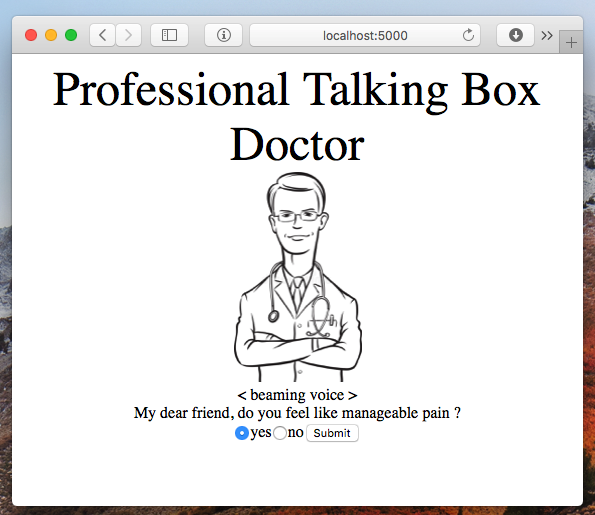
\includegraphics[scale = 0.4]{report_img/ScreenShot1.png}
  \caption{Question 1}
  \label{ss1}
\end{figure}
\begin{figure}[H]
    \centering
  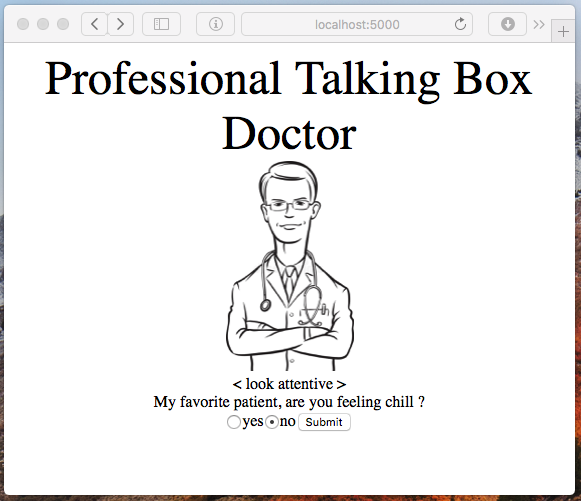
\includegraphics[scale = 0.4]{report_img/ScreenShot2.png}
  \caption{Question 2}
  \label{ss2}
\end{figure}
\begin{figure}[H]
    \centering
  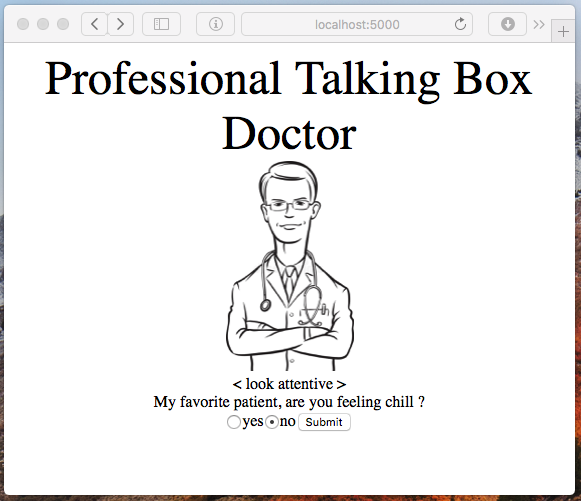
\includegraphics[scale = 0.4]{report_img/ScreenShot2.png}
  \caption{Result}
  \label{ss3}
\end{figure}

\end{document}
